
\documentclass[a4paper,12pt]{report} %define [paper and default font size]{report or article}
%----------------set borders ---------------------------------
\usepackage[left=35mm, right=25mm, top=25mm,bottom=25mm]{geometry}
%\usepackage{times} % default times new roman font
\usepackage{newtxmath,newtxtext}% alternative times new roman font if needed uncomment
\usepackage{amsmath} % for equations and symbols

%-------hypenation of words at end avoiding block----%
\tolerance=1
\emergencystretch=\maxdimen
\hyphenpenalty=10000
\hbadness=10000

%-------------------Line spacing------------------------------%
\usepackage{setspace} 
\linespread{1.5} 
%----change name bibliograpy to references---%
\renewcommand\bibname{References}
% Set the right side of the footer to be the page number
%\fancyfoot[R]{\thepage}'
%\fancypagestyle{report}{%
% \renewcommand{\headrulewidth}{0pt}%
%\fancyhf{} %clear all headers and footers fields
%\fancyfoot[R]{\thepage} %prints the page number on the right side of the header
%}

%------------ for setting the page number to right bottom--------------------%
\usepackage{fancyhdr}
\fancypagestyle{plain}{%
    \renewcommand{\headrulewidth}{0pt}%
    \fancyhf{}%
    \fancyfoot[R]{\thepage}%
}
\fancyhf{} % clear all header and footers
\renewcommand{\headrulewidth}{0pt} % remove the header rule
\rfoot{\thepage}
\pagestyle{fancy}

%-----------------for roman numerals at first and arabic afterwards defined front and mainmatter-----%
\newcommand\frontmatter{%
    \cleardoublepage
  %\@mainmatterfalse
  \pagenumbering{roman}}

\newcommand\mainmatter{%
    \cleardoublepage
 % \@mainmattertrue
  \pagenumbering{arabic}}

\usepackage{enumitem} % for bullets and numbers
\usepackage{graphicx} % for inserting figures

%---- for putting chapter name in CAPS and then right aligning them-----%
\usepackage{sectsty}
\renewcommand{\chaptername}{CHAPTER}
\chapterfont{\raggedleft}

%\usepackage{titlesec}


% -----------------for intending every paragraph-------------------------%

\usepackage{indentfirst}
 \setlength{\parindent}{10mm}

%--------------------- for bold captions for figures -------%
 \usepackage{caption}
  \captionsetup[figure]{format=hang,labelfont={bf},name={Fig.},labelsep=period,textfont={bf}}
  
  
  \setcounter{tocdepth}{4}
\setcounter{secnumdepth}{4}

\usepackage{tocbibind}
%\addcontentsline{toc}{chapter}{List of Symbols}

\begin{document}

%\title{Understanding Latex for Beginners}
%\author{Vetri}
\frontmatter
\pagenumbering{roman}

%\maketitle
\begin{titlepage}
   \begin{center}
%       \vspace*{1cm}
 
   \Large
   {\textbf{SIGNAL PROCESSING ALGORITHM FOR
RESTORATION OF CLIPPED SIGNAL IN SPEECH RECOGNITION SYSTEM}}\\
 \large
       \vspace{0.5cm}
        \textbf{18CN280 Project Report }
 
   \vspace{1cm}
  \large
    \textit{Submitted in partial fulfillment for the requirement of M.E. degree in\\
        Communication Systems of Anna University}\\
         \vspace{0.75cm}
  \textit{Submitted by}\\
       \textbf{J.JOHN SMITH}\\
       \textit{\textbf{Reg. No:18N099}}\\
          \vspace{0.5cm}
         \textit{Guided by}\\
       \textbf{Dr. ABDUL KALAM M.E.,Ph.D.}\\
 
       \vfill
 
%       \vspace{0.8cm}
 
       
\includegraphics[width=0.3\textwidth]{TCE}\\
  \large\textit{\textbf{Department of\\ Electronics and Communication Engineering}}\\
      \Large\textbf{THIAGARAJAR COLLEGE OF ENGINEERING}\\
       \normalsize (An Autonomous Institution Affiliated To Anna University, Chennai)\\
        \Large\textbf{MADURAI - 625015}\\
       \large \textbf{May 2020}
 
   \end{center}
\end{titlepage}
\thispagestyle{plain}
\begin{center}
     \Large\textbf{THIAGARAJAR COLLEGE OF ENGINEERING}\\
       \normalsize (An Autonomous Institution Affiliated To Anna University, Chennai)\\
        \Large\textbf{MADURAI - 625015}\\
       \large \textbf{May 2020}\\
   
\includegraphics[width=0.2\textwidth]{TCE}\\
    \vspace{0.3cm}
    \large
   \Large\textbf{BONAFIDE CERTIFICATE}
   
\end{center}
\normalsize

   This is to certify that the 18CN280 Mini Project entitled “SIGNAL PROCESSING ALGORITHM FOR RESTORATION OF CLIPPED SIGNAL IN SPEECH RECOGNITION SYSTEM”, being submitted by J.JOHN SMITH (Register Number 18N099) in partial fulfillment for the requirement of Master of Engineering Degree in Communication Systems, is a record of bonafide work done by her during the year 2018-2019 under my supervision. The results embodied in this report have not been submitted to any other university or institute for the award of any degree or diploma.\\\\\\
 \hfill
 Dr. ABDUL KALAM M.E.,Ph.D.
 \hfill
Dr. S.J.Thiruvengadam, M.E., Ph.D. \\
 Associate Professor
 \hfill Professor and Head\\
 Department of ECE
 \hfill  Department of ECE\\
 (Guide)\\
 Station:Madurai\\
 Date:\today
\par\noindent\rule{\textwidth}{0.4pt}
 Certified that the Candidate was examined in the Viva-Voce Examination held at Thiagarajar College of Engineering, Madurai on \_\_\_\_\_\_\_\_\_\_\\\\
 
\noindent INTERNAL EXAMINER \hspace{1.5cm} EXTERNAL EXAMINER \hspace{1.5cm}HOD ECE
\chapter*{ACKNOWLEDGEMENT}
I would like to express my wholehearted gratitude to our management
for provided me with all facilities to build my project successfully. I express
my sincere thanks to \textbf{Dr. KARUMUTTU T. KANNAN}, Chairman and
Correspondent, Thiagarajar College of Engineering, for providing me with
required amenities.\par
I extend my gratitude to \textbf{Dr. V. ABHAIKUMAR}, Principal,
Thiagarajar College of Engineering, for his inspiring help, support and
guidance to follow the right direction for completing this project.\par
I express my extreme gratefulness to \textbf{Dr. S. J. THIRUVENGADAM},
Professor and Head of the department of Electronics and Communication
Engineering, for his constant support and encourage coming out with new
ideas.
%\addcontentsline{toc}{chapter}{Title}
%\addcontentsline{toc}{section}{ACKNOWLEDGEMENT}
%\addcontentsline{toc}{section}{List of published papers}

%\addcontentsline{toc}{chapter}{List of Symbols}
\tableofcontents
\makeatother

%\tableofcontents
\listoffigures
\listoftables
\chapter*{List of Symbols}
\begin{tabular}{cp{0.6\textwidth}}
  $x$ & position \\
  $v$ & velocity \\
  $a$ & acceleration \\
  $t$ & time \\
  $F$ & force
\end{tabular}\\
\chapter*{List of Abbreviations}
\begin{tabular}{cp{0.6\textwidth}}
  SMS & Short Messaging Service \\
  5GEx & 5G Exchange \\
  SoC & Silicon on Chip \\
  QAM & Quadrature Amplitude Modulation \\
  F & force
\end{tabular}\\
%\newpage
\mainmatter

%\cleardoublepage
\pagenumbering{arabic}
\chapter{INTRODUCTION}
\section{INTRODUCTION}

speech has always been the fundamental mode of communication~\cite{Devi2017} and in case of human-machine interaction~\cite{Suresh2017}, spoken language has been accepted as the natural method~\cite{Manikandan2012}. Our ability to communicate with machines and computers is far more difficult and slower in magnitude when carried out through keyboards, mouse and other devices~\cite{Rajkumar2017}. Thus speech input is an essential component in order to make this communication more user friendly~\cite{K2017} ~\cite{Maheswari2017}. Besides, a great deal of information is expressed by humans by means of natural speech. Thus even an illiterate or a person with little knowledge about computers can operate computers using speech commands.Among humans\cite{adler2011}, .\par
\textbf{\textit{h}}
Many physically disabled people in case they are unable to type in keyboard or click in mouse with their hands may use computers with the help of speech input. People who have sufficient expertise with computers can utilize the speech input ability of a computer to significantly speedup documentation, writing e-mail sending and other significant operations using computers. Also there are many advantages to this mode of operation such as it can be used for many situations when the hands are already being used for other important operations such as driving a car. Two good examples for speech based system are speech enabled dialing and Global Positioning System. Another exciting application called Automatic Spoken Language Translation had emerged with the development of Machine Translation techniques. This allows people from different countries all over the world to communicate freely without any professional translator via speech. \par
\begin{table}[]
\centering
\begin{tabular}{|l|l|l|ll}
\cline{1-3}
\textbf{SNO} & \textbf{SYNTAX}         & \textbf{OUTCOME} &  &  \\ \cline{1-3}
1            & $\eta$     & just symbols     &  &  \\ \cline{1-3}
2            & $\pi$      & 22 7             &  &  \\ \cline{1-3}
3            &$ \epsilon$ & ee               &  &  \\ \cline{1-3}
\end{tabular}
\caption{just a table sample}
\end{table}
Speech processing applications are usually focused on the problem of analyzing an electrical signal and understanding the information content from the speech of a particular speaker. For example, in a recording of a meeting consisting of ten speakers, it may be necessary to perform automatic speech recognition(ASR), and also label the speech as coming from a specific speaker among the ten present, i.e., speaker identification (SID). In such scenarios where machines are required to perform the tasks of recognizing who spoke what, it becomes necessary to first separate the incoming mixture of various sources from each other, and then follow each individual speech stream with the relevant task. Furthermore, many real-world situations consist of speech signals which are interspersed is with various forms of distortion, like noise from multiple sources as well as background speech from speakers other than the primary speaker.\par
Thus, the task becomes more difficult, as there is also a need to enhance the quality of the speech by removing the background noise. The task of separation of speech from noise or a background speaker has been looked at by researchers for several years, and most approaches focus on exploiting the mutual information arising from a set of sensors/microphones. The approach has been to capture the mixture speech (i.e. from multiple speakers) or noisy speech using more than one microphone, and then designing optimal weights to combine the outputs of these microphones, so as to maximize the quality of the reconstructed individual speaker’s speech. Each microphone functions like an antenna with a beam in a certain direction, and these beams can be combined in certain ways. The weights of these various microphones are designed in such a way, that the collective beam of all the microphones is directed towards the primary speech of interest and the background signal escapes very weakly into this collective beam. Multi-microphone approaches of this kind are collectively called Optimal Antenna Beam-forming. An important drawback of this approach is that the direction of the target speech must be known beforehand, so that the antenna beam may be formed to point in the desired direction. Several other techniques fall under the category of Blind Source Separation (BSS), Independent Component Analysis (ICA) etc., and these methods work by exploiting the signals from multiple microphones to hypothesize signals which are statistically more independent from each other and presumably gave rise to the observed mixtures. For the BSS and ICA methods in practice, the number of sensors (microphones) must typically be equal to the number of speakers to ensure good separation of the speech signals.   

\section{SPEECH SIGNAL}
Speech is the most common \& primary mode of communication among human beings. It is the most natural and efficient form of exchanging information among humans. Human voice conveys much more information such as gender, emotion and identity of the speaker. Speech Recognition can be defined as the process of converting speech signal to a sequence of words by means an Algorithm. Speech is composed of a sequence of sounds and the sounds when shared between humans serves as a symbolic representation of information. In a medium, such as air or water, speech propagates as a longitudinal wave. Depending on the density of the medium the speed of propagation varies. Commonly the amplitude of air pressure variation corresponding to a speech signal is plotted as a function of time. This kind of plot is known as a speech pressure waveform or just a speech waveform as shown Figure \ref{fig1}
\begin{figure}
\begin{center}
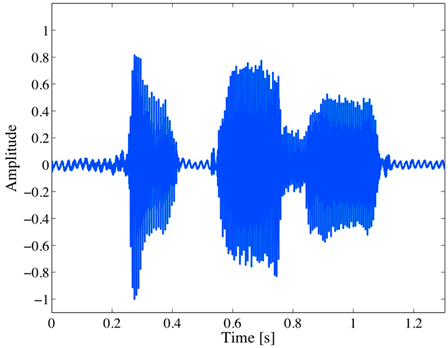
\includegraphics[width=0.6\linewidth]{figure1}
\caption{Speech waveform in time}
\label{fig1}
\end{center}
\end{figure}
\subsection{Properties of Sinusoids}
A sinusoid corresponds to a time waveform drawn with a simple smooth up and down movement. There are three kinds of measurement that can be taken from a sinusoid that can completely define the shape of a waveform when they are taken into account together. 
\subsubsection{Amplitude}
Size of the displacement above and below the mid line of a sinusoid. This signifies the energy in the sound wave and it corresponds to loudness of the sound wave. Amplitude can be measured in many ways; it can be measured in units of pressure as it is related to the size of the pressure variations in the air. More often we measure amplitude on a logarithmic scale called deciBels (dB) which is relative to a standard sound. The dB scale maps directly to the way that humans perceive loudness and hence is found to be very useful form of measure. 
\subsubsection{Frequency}
The number of cycles the sinusoid makes in each second can be termed as the frequency. A cycle consists of an oscillation from the mid line to the maximum, down to the minimum and back to the midline. Frequency is measured in Hertz (Hz) or in other words simply cycles per second. 
\subsubsection{Phase}
The position of the starting point of the sinusoid is termed as Phase. The phase of those starting at the maximum is said to be zero while a phase of $\pi$ radians is considered to be for those starting at the minimum. Perceiving the phase of a sinusoid is not possible but the relative changes in phase between two signals can be detected, as the brain determines the location of a sound on the basis of different phases heard at the two ears forms the basis of binaural hearing.

\subsection{Properties of speech signal }
Significant energy is present in speech ranging from zero frequency up to around 5 kHz. The speech signal properties changes remarkably as a function of time. The concept of time varying Fourier representation is used to study the spectral properties of speech signal. However, the temporal properties of speech signal such as energy, correlation, zero crossing etc are assumed to remain constant over a short period. That is its characteristics are short-time stationary .Therefore, Speech signal is divided into a number of short duration blocks using hamming window, so that normal Fourier transform can be used. Some of the important properties of speech signals are summarized as follows. 
\subsubsection{Bandwidth}
The speech signal has a bandwidth much higher than 4 kHz. In fact, there is still a significant amount of energy in the spectrum for high and even ultrasonic frequencies for the fricatives. However, as we all know from using the (analog) phone, it seems that the speech signal contains all the information necessary to understand a human voice within a bandwidth of 4 kHz. 
\subsubsection{Fundamental Frequency }
The usage of voiced excitation for the speech sound results in a pulse train, which is termed as fundamental frequency. The signal has a fundamental frequency between 80 Hz and 350 Hz and is periodic in nature. While voiced excitation is normally used in case of articulating vowels and some of the consonants, unvoiced excitation (noise) is used for fricatives (e.g. /s/ as in mess, or /f/ as in fish). Usually no fundamental frequency can be detected in such cases. On the other hand, the signal has very high zero crossing rate. Plosives(like /p/ as in put),that uses transient excitation can be best detected in the speech signal by looking for the short silence necessary to build up the air pressure before the plosives are bursted out. 
\subsubsection{Peaks in the Spectrum}
The vocal tract gives a characteristic spectral shape to the speech signal after passing the glottis. If one simplifies the vocal tract to a straight pipe (approximately of 17cm length), one can see that the pipe shows resonance at certain frequencies. These frequencies are called formant frequencies. The frequency of the formants (especially of the 1st and 2nd formant) change depending on the shape of the vocal tract (the diameter of the pipe varies along the pipe), and therefore the vowel being articulated is characterized. The peaks in the spectral distribution of energy is given by (2n $-$ 1) *500 Hz; Where n =1, 2, 3,..,
\section{SPEECH CODING}
Speech coding is the field concerned with compression and decompression of the digital information necessary to represent a speech signal. Digital speech brings flexibility but it is also associated with a high data rate. The objective of speech coding is represent speech with a minimum bit rate its perceptual quality. Speech coders compress signals by exploiting the natural redundancies in speech and the properties of human hearing. Most compression techniques used in speech coding are known as lossy compression where the reproduced speech is not identical to the original. The signal, however, sounds like the original because of the masking properties of human ear that render a level of certain types of noise inaudible. Speech coder is used to transmit and store speech for various applications. Examples of transmission applications include wireless cellular, satellite communications, internet phone, audio and video conference, and secure voice systems. In particular, wireless cellular and satellite communications have been enjoying a tremendous worldwide growth. Storage applications include digital telephone answering machines, voice-mail, Text-to-Speech (TTS) systems.\par
Digital coding of speech signals can be broadly classified into three categories namely Analysis –synthesis (vocoder) coding, waveform coding and hybrid coding. The concepts used in the first two methods are very different, and the third method is a mixture of the first two coding systems. In the vocoding systems only the theoretical model of the speech production mechanism is considered and its parameters are derived from the actual speech signal and coded for transmission. At the receiver these modal parameters are decoded and used to control a speech synthesizer which corresponds to the model assumed in the analyzer. Provided that the perceptually significant parameters of the speech are extracted and transmitted, the synthesized signal perceived by the human ear approximately resembles the original speech signal. Therefore, during the analysis procedure the speech is reduced to its essential features and all of the redundancies are removed.\par Consequently a great saving in transmission bandwidth is achieved. However, when compared with the waveform coding methods, analysis –synthesis processing operations are complex, resulting in expensive equipment. In waveform coding systems an attempt is made to preserve the waveform of original speech signal. In such a coding system the speech waveform is sampled and each sample is coded and transmitted. At the receiver the speech signal is reproduced from the decoded samples. The way in which the input samples are coded at the transmitter may depend upon the previous samples or parameters derived from the previous samples so that advantage of the speech waveform characteristics can be taken. Waveform coding systems tend to be much simpler and therefore inexpensive compared to the vocoder type systems.
\section{SPEECH PRODUCTION}
Speech production takes place by means of the biological system of a larynx or sound box, which resides in the throat of the human beings .The fibers provided in the larynx or the sound box are capable of vibrating when the air passes through them. The lung, attached to the larynx, by the windpipe, is the major organ that pumps air through the larynx. The laryngeal fibers or vocal cords are properly capable of vibrating at all frequencies. The range goes from the just audible 20 Hz up to about 11000 Hz in some particular case. The higher frequencies are usually found in children and women while the lower frequencies are found in men.\par 
 In terms of Signal Processing, the larynx can be called as the source and vocal tract as the filter .The Source is capable of vibrating at many or may be at all frequencies . The vocal tract which includes the vocal cavity, the mouth cavity \& the nasal cavity, filters the sound thus produced to resonate some frequencies \& anti resonates others so that a special sound emanates from the lips in the form of speech.\par 
The length and shape of the vocal tract do not change constantly but remains stable over a scale of millisecond. Hence the characteristics of the filter are stable over the millisecond scale of the millisecond. Thus on small scale a person’s voice has a static nature and on a larger scale has a dynamic nature.\par 
Every time when the speech sounds are produced, the air flowing from lungs first passes through the glottis and then the throat and mouth. The speech signal can be excited in three possible ways depending on the speech sound which is being articulated by the speaker.
\subsection{Voiced excitation}
The air pressure forces the glottis, which is initially in the closed condition, to open and close periodically there by generating a periodic pulse train (triangle–shaped). This fundamental frequency usually lies in the range from 80Hz to 350Hz. 
\subsection{Unvoiced excitation}
The glottis is in the open state and the air passes through a narrow passage in the throat or mouth. This results in a turbulence which results in generating a noise signal. The location of the narrowness determines the spectral shape of the noise. 

\subsection{Transient excitation}
 The air pressure is raised due to a closure in the throat or mouth. The air pressure drops down immediately by suddenly opening the closure. With some speech sounds these three kinds of excitation occurs in combination. The shape of the vocal tract determines the spectral shape of the speech signal. You change the spectral shape of the speech signal by changing the shape of the pipe (and opening and closing the air flow through your nose) and thus different speech sounds are articulated.
 
 \section{SPEECH RECOGNITION }
 Speech Recognition is a special case of pattern recognition. The process of converting speech signal to a sequence of words by means of algorithm implemented as a program is called speech recognition. The goal of speech recognition is to provide machine with the ability to "hear,” understand," and "act upon" spoken information. Figure 1.2 shows that the  Speech recognition phases consists of training and testing phase. In both phases, the process of extraction of features relevant for classification is common. The parameters of the classification model are estimated using a large number of class examples (Training Data) during the training phase. The feature of test pattern (test speech data) is matched with the trained model of each and every class during the testing or recognition phase. The test pattern is declared to belong to that model which matches the test pattern in the best way.
 \subsection{Classification of Speech recognition systems }
 \subsubsection{Based on types of Speech Utterance}
          An utterance is the vocalization (speaking) of a word or words that represent a single meaning to the computer. A single word, a few words, a sentence, or even multiple sentences may be considered as an utterance. The types of speech utterances are: 
\paragraph{Isolated Words}
          Usually isolated word recognizers require to have quiet on both sides of the sample window for each utterance. It doesn't mean that it accepts single words alone, but a single utterance at a time is a prerequisite. Though the system proves to be effective for situations where the user requires to give only one word responses or commands, it is very unnatural for multiple word inputs. Since word boundaries are obvious and the words tend to be clearly pronounced, it is comparatively far more simpler and easier to implement. 
 \paragraph{Connected Words}
        Though connected word systems (or more correctly 'connected utterances') are somewhat similar to isolated words, they allow separate utterances with minimal pause in between to be 'run-together'.
\paragraph{Continuous Speech}
Continuous speech recognizers allow users to speak almost naturally, while the computer determines the content. In other words, it's basically computer dictation. It includes a great deal of "co articulation", in which adjacent words run together without any apparent division or pauses in between. As continuous speech recognition systems must utilize special methods to determine utterance boundaries, they are comparatively most difficult to create. Confusability between different word sequences grows as vocabulary grows larger.
\paragraph{Spontaneous Speech}
This kind of speech is natural and not rehearsed. A variety of natural speech features such as words being run together and even slight stutters should be handled by an ASR system with spontaneous speech. Spontaneous (unrehearsed) speech includes false-starts, mispronunciations and non-words.
\subsubsection{Based on the type of Speaker Model}
        Due to one’s unique physical body and personality all speakers have their special voices. Based on speaker models, speech recognition system is broadly classified into two main categories namely speaker dependent and speaker independent.
 \paragraph{Spontaneous Speech}
           This kind of speech is natural and not rehearsed. A variety of natural speech features such as words being run together and even slight stutters should be handled by an ASR system with spontaneous speech. Spontaneous (unrehearsed) speech includes false-starts, mispronunciations and non-words.
\subsubsection{Based on the type of Speaker Model}
        Due to one’s unique physical body and personality all speakers have their special voices. Based on speaker models, speech recognition system is broadly classified into two main categories namely speaker dependent and speaker independent.
\paragraph{Speaker dependent models}
Speaker dependent systems are designed for a specific speaker. For a particular speaker they are generally more accurate, but much less accurate for other speakers. Though these systems are usually cheaper, easier to develop and more accurate they are comparatively not as flexible as speaker adaptive or speaker independent systems.
\paragraph{Speaker independent models}
Speaker independent systems are designed for supporting a variety of speakers instead of a specific one. It can recognize the speech patterns of a large group of people. But unlike speaker dependent systems this system is more difficult to develop, more expensive and offers comparatively lesser accuracy. However, they are more flexible
\subsubsection{Based on types of Vocabulary }
        The complexity, processing requirements and the accuracy of the system is greatly affected by the size of the vocabulary of a speech recognition system. Where some applications only require a few words (e.g. numbers only), others require very large dictionaries (e.g. dictation machines). 
\section{APPLICATIONS OF SPEECH RECOGNITION}
Today, speech recognition systems find widespread application in tasks that requires human machine interface. Speech recognition can be applied in applications such as railway reservations, query based information systems that provide updated travel information, , weather reports, access to information: travel, banking, Commands, Avionics, Automobile portal, speech transcription, voice dictation, handicapped people (blind people) supermarket, stock price quotations, automatic call processing in telephone networks, data entry etc. Within telephone networks, speech recognition technology was increasingly used in automation as well as to enhancing the operator services.
\section{SPEECH ENHANCEMENT}
Speech enhancement deals with processing of noisy speech signals, aiming at improving their perception by human or their correct decoding by machines. Speech enhancement algorithms attempt to improve the performance of communication systems when their input or output signals are corrupted by noise. The presence of background noise causes the quality and intelligibility of speech to degrade. Here, the quality of speech refers how a speaker conveys an utterance and includes such attributes like naturalness and speaker recognizability. Intelligibility is concerned with what the speaker had said, that is, the meaning or information content behind the words. Therefore, a noisy environment reduces the speaker and listeners ability to communicate. To reduce the impact of this problem speech enhancement can be performed. It is usually difficult to reduce noise without distorting speech and thus, the performance of speech enhancement systems is limited by the tradeoff between speech distortion and noise reduction.\par
Efforts to achieve higher quality and/or intelligibility of noisy speech may effectively end up improving performance of other speech applications such as speech coding/compression and speech recognition, hearing aids, voice communication systems and so on. The goal of speech enhancement varies according to specific applications, such as to reduce listener fatigue, to boost the overall speech quality, to increase intelligibility and to improve the performance of the voice communication device. Hence speech enhancement is necessary to avoid the degradation of speech quality and to overcome the limitations of human auditory systems.
\section{COMMON SOURCES OF NOISE}
For communication systems, two general objectives depend on the nature of the noise and often on the signal to noise ratio (SNR) of the distorted speech. With medium to high input SNR, reducing the noise level can produce a subjectively natural speech signals at a receiver or can obtain reliable transmission. For low SNR, the objective could be to decrease the noise level, while retaining or increasing the intelligibility and reducing the fatigue caused by heavy noise for example motor and street noise. Figure 1.3 shows the factors that affect the speech signal during transmission at various stages by different noise sources. Sources that degrade speech quality are noisy environment during acquisition, background noise, multi-speaker effect, noisy transmission channel and imperfect speech reproduction. In the transmission side the effect of background noise are added with the desired signal and the signal from other speakers are treated as noise for the desired speaker. The signal with background noise is transmitted through the channel where the transmission channel noise is also added with the desired signal.

\chapter{LITERATURE REVIEW}
\begin{enumerate}[listparindent=10mm]
\item \textbf{Jonathan S. Abel Julius O. Smith, “Restoring a clipped signal”, IEEE International Conference on Acoustics, Speech, and Signal Processing, vol.3, pp. 1745-1748, 1991.}

The restoration of a band-limited signal which has under- gone amplitude clipping is studied. This problem can be viewed as that of recovery from signal drop-outs with the extrapolated signal constrained to lie outside the clipping interval during the drop out. If the signal is oversampled, and the clipping threshold moderate, a unique reconstruction often results from application of signal matching and bandwidth constraints. In light of this finding, methods for choosing a unique reconstructions are discussed. Finally, the case of noise is considered.

\item \textbf{J. Serignat, L. Besacier, P. Mayorga, R. Lamy , “Audio packet loss over IP and speech recognition”, IEEE Workshop on Automatic Speech Recognition and Understanding , pp. 607-612, 2003}

This paper deals with the effects of packet loss on speech recognition over IP connections. The performance of  continuous French speech recognition system is here evaluated for different transmission scenarios. A packet loss simulation model is first proposed in order to simulate different channel degradation conditions. The packet loss problem is also investigated in real transmissions through IP. Because packet loss impact may be different according to the speech coder used to transmit data, different transmission conditions with different audio codecs are also investigated. Several reconstruction strategies to recover lost information are then proposed, and tested. Another solution for dialog applications is also suggested, where the relative weight of language and acoustic model is changed according to the packet loss rate. The results show that the speech recognition performance can be augmented by the solutions here presented.

\item \textbf{M. S. Scordilis ,Wen Jin, “Speech enhancement by Kalman filtering with residual noise clipping”, Proceedings. IEEE, pp. 225-228, 2005}

In this paper, an improved speech enhancement system based on Kalman Filtering (KF) that processes the linear prediction (LP) residual of voiced speech was developed. For input frames where voiced speech is present, the LP residuals are clipped to maintain the peaks where the major excitation pulses are located. The proposed algorithm differs from the conventional Kalman Filtering algorithms in that it includes this quasi-periodic term in the process equation for voiced speech frames. The quality of the resulting enhanced speech is evaluated by means of Signal-to-Noise-Ratio (SNR) and ITU-PESQ scores. Experimental results indicate that the proposed algorithm achieves consistent improvement in output speech quality when compared to conventional KF methods.
\end{enumerate}

\chapter{RESULTS AND DISCUSSIONS}

Experimental results indicate that the proposed algorithm achieves consistent improvement in output speech quality when compared to conventional KF methods.samples for equations,
\begin{equation}
s(t)=\sum_{n=-\infty}^{\infty} \sum_{m=0}^{N-1} i^{m+n} x_{m, n}^{\prime} \cdot \operatorname{rect}(t-n T / 2) e^{i 2 \pi m t / 2}
\end{equation}
how does it look
\begin{equation}
s(t)=\sum_{n=-\infty}^{\infty} i^{n} \Im(t-n T / 2) \cdot X_{n}^{\prime \prime}(t)
\end{equation}
these are from FTN book
\begin{equation}
\frac{N_{\mathrm{FTN}} \times M_{\mathrm{FTN}}}{N \times M} \rightarrow \frac{1}{T_{\Delta} F_{\Delta}}
\end{equation}
i use a mathpix snipping tool 
\begin{equation}
\overline{x}_{k, \ell}=\sum_{m, n} H_{m}^{*} C_{k, \ell, m, n}\left(H_{m} \sum_{k_{p}, \ell_{q}} x_{k_{p}, \ell_{q}} C_{k_{p}, \ell_{q}, m, n}\right)+\eta_{k, \ell}^{\prime}
\end{equation}

\bibliographystyle{IEEEtr}
\bibliography{bibbo}
\end{document}
